\section{Introduction}
\label{sec:introduction}

Driven by its clean nature and reliable supply, wind power has become an important energy source for modern power systems. Accurate short-term forecasts of wind speed and wind direction support grid dispatch, resource allocation, and wind-energy utilization \cite{Hanifi2020CriticalReviewWindPowerForecasting,Jung2014CurrentStatusWindSpeedPowerForecasting}. In a wind farm, however, these variables are not homogeneous multivariate channels. They are shaped by different physical structures across turbines and also have different mathematical properties \cite{Chen2014WindPowerForecastsGaussianProcesses,Dolatabadi2022DeepSpatialTemporal2DCNNBLSTM}. A forecasting model should therefore share information selectively rather than imposing one interaction pattern on every wind variable.

\begin{figure}[htbp]
\centering

\includegraphics[width=0.9\textwidth]{figures/figure1.png}
\caption{Conceptual contrast between shared but non-identical wind-speed dynamics and turbine-specific wind-direction variation.}
\label{fig:data_properties}
\end{figure}

\subsection{Challenge 1: Shared but Non-identical Wind-Speed Dynamics}
\label{subsec:speed_sharing_intro}

Wind turbines in the same farm are driven by common weather processes and large-scale incoming flows, so their wind-speed trajectories often exhibit synchronized trends. At the same time, local terrain, wake effects, and turbine positions produce turbine-level deviations. This combination creates a structural tension: channel-independent methods preserve local freedom but repeatedly relearn common variation, whereas fully correlated methods may mix common dynamics and local deviations in a single representation. The key challenge is therefore to share the common wind field while retaining turbine-specific residual information.

Figure~\ref{fig:speed_multiscale_similarity} provides supporting evidence for this view. Representative turbines exhibit similar dominant spectral components and wavelet-energy patterns, suggesting a shared temporal scaffold rather than a collection of unrelated sequences. The remaining differences motivate a separate residual branch instead of assuming that all turbines are identical.

\begin{figure}[htbp]
\centering
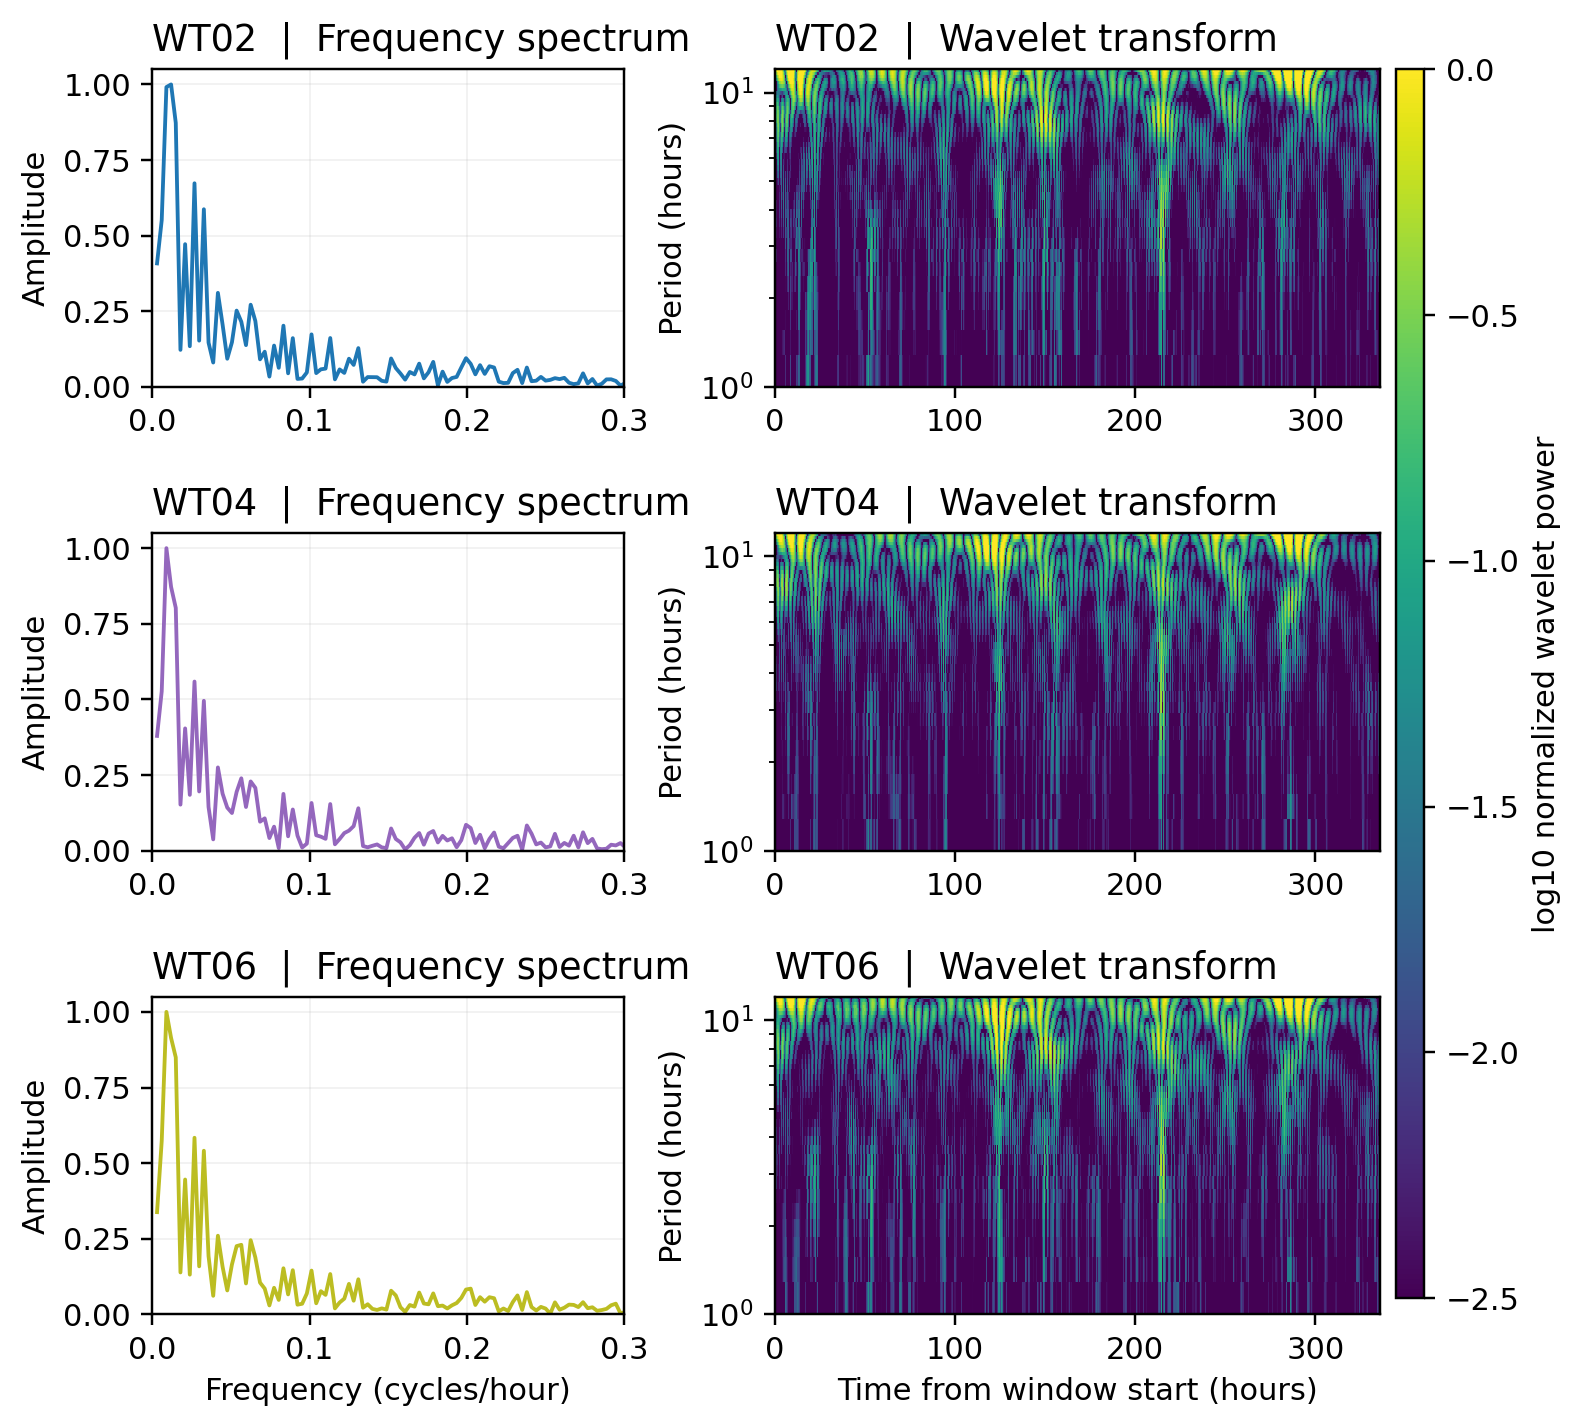
\includegraphics[width=0.9\textwidth]{figures/figure2.png}
\caption{Frequency-spectrum and wavelet-transform comparison of representative turbine wind-speed sequences. Similar dominant components support a shared temporal scaffold, while turbine-level deviations motivate residual modeling.}
\label{fig:speed_multiscale_similarity}
\end{figure}

After separating the shared component, the common wind-speed history still needs an effective temporal organization. Rather than treating a screened candidate scale as a strict physical period, we organize the history by candidate temporal scales and relative phase positions within temporal blocks. This phase-aware organization allows local dynamics at comparable positions across blocks to interact.

\subsection{Challenge 2: Turbine-specific and Circular Wind Directions}
\label{subsec:direction_2d_intro}

Wind direction follows a different cross-turbine structure. Interactions among turbine locations, wake effects, and local flow fields cause different units to exhibit distinct dominant directions and turning patterns, so direction should not be collapsed into a common representation in the same way as wind speed. Figure~\ref{fig:direction_specificity} (a) shows that the dominant directions and directional concentration levels of different turbines are not consistent. Figure~\ref{fig:direction_specificity} (b) reports that about 51\% of turbine pairs have an average angular distance of no less than $90^\circ$, indicating that the heterogeneity is not caused by a few isolated units. Figure~\ref{fig:direction_specificity} (c) further displays structured variation in the pairwise angular-distance matrix. These observations motivate turbine-wise direction modeling.

\begin{figure}[htbp]
\centering

\includegraphics[width=0.9\textwidth]{figures/all_24_turbines_direction_difference_summary.png}
\caption{Turbine-specific wind-direction distributions and all-pair angular differences among 24 turbines.}
\label{fig:direction_specificity}
\end{figure}

Wind direction is also a circular variable rather than an ordinary one-dimensional scalar. It satisfies

\begin{equation}
\theta \equiv \theta+360^\circ.
\end{equation}

Consequently, $359^\circ$ and $1^\circ$ are physically close even though their scalar difference is $358^\circ$. Direct scalar regression can therefore create artificial discontinuities in distances, local variations, and error gradients. To preserve this geometry from input to prediction, WindFormer maps each direction angle into a two-dimensional sine-cosine unit vector:

\begin{equation}
\mathbf{u}_{t,n} = [\cos(\theta_{t,n}), \sin(\theta_{t,n})].
\end{equation}

The model predicts in this continuous representation, applies direction-vector and wind-vector consistency constraints, and recovers the angle using

\begin{equation}
\hat{\theta}_{t,n} = \operatorname{atan2} \left( \hat{u}^{\sin}_{t,n}, \hat{u}^{\cos}_{t,n} \right).
\end{equation}

Because directional patterns remain turbine-specific, each turbine is processed as an individual two-dimensional sequence. The temporal patch projection and Patch-Attention encoder are shared across turbines, allowing transferable local dynamics to be learned without collapsing distinct directional distributions into one global state.

\subsection{WindFormer Framework}

The two challenges lead to a single design principle: share information where the wind field is physically common, preserve information where turbine behavior is specific, and keep the direction representation geometrically valid. WindFormer implements this principle with two representation-decoupled branches and one objective-level coupling mechanism. The wind-speed branch extracts a learnable common field, models it with Phase-Attention organized by screened candidate temporal scales, and reconstructs turbine forecasts from the common prediction and shared residual predictors. The wind-direction branch retains each turbine's sequence, maps angles to sine-cosine components, and uses shared Patch-Attention to forecast future direction vectors. The branches are trained jointly through wind-speed, direction-vector, and wind-vector consistency losses.

The main contributions of this paper are as follows:

\begin{itemize}
    \item \textbf{We separate shared and local wind-speed dynamics.} A learnable aggregation extracts shared wind-speed dynamics, while a shared residual branch restores turbine-level deviations. A phase-aware temporal encoder organizes the common history by screened candidate scales and relative positions rather than assuming a strict physical period.
    \item \textbf{We develop a turbine-wise circular direction branch within the same forecasting framework.} Sine-cosine vectors preserve boundary continuity, and shared Patch-Attention captures transferable temporal patterns while retaining turbine-specific directional sequences.
    \item \textbf{We couple the two task-specific branches through a physical wind-vector objective and evaluate the resulting WindFormer framework comprehensively.} Standard forecasting, component ablations, robustness tests, sparse-deployment transfer, efficiency measurements, and matched-seed statistical tests together assess accuracy, mechanism, stability, and generalization.
\end{itemize}

\section{Related Work}
\label{sec:related_work}

\subsection{Spatial Relationships in Multi-Turbine Wind Power Forecasting}

Existing deep learning studies usually improve wind forecasting by modeling spatial relationships among turbines. Graph-based and convolutional recurrent models encode turbine topology, neighborhood influence, multi-scale spatial dependence, or local and long-range interactions into the forecasting process \cite{Song2023ShortTermForecastingGraphConvolutionWindPower,Zhang2019LSTMNeighborhoodGatesCausalityWindSpeed,Wu2024MixFormerHierarchicalContextWindSpeed}. To handle condition-dependent relationships, later studies further introduce channel-aware dependence and temporal lead-lag structures \cite{Zhao2024RethinkingChannelDependenceLeadingIndicators,Zhu2024GGNetTemporalLeadLagCorrelations}. These methods show that cross-turbine information is useful for short-term wind forecasting.

Generic multivariate time-series models also provide useful designs for organizing turbine variables. PatchTST reduces cross-channel interference through channel-independent temporal modeling \cite{Nie2023PatchTST}, TimesNet converts temporal variations into two-dimensional period structures \cite{Wu2023TimesNetTemporal2DVariationModeling}, iTransformer learns dependencies along the variable dimension \cite{Liu2024iTransformer}, and MSGNet enhances multi-scale cross-sequence interaction \cite{Cai2024MSGNetLearningMultiScaleInterSeriesCorrelations}. MST-Net further discusses the combination of channel-independent and spatially correlated modeling for short-term wind resource forecasting \cite{Lou2026MSTNet}. More recently, an Information Sciences study further explores a global-local dual-branch design and pyramid patch interaction for multivariate forecasting \cite{Zhou2026GLPTGlobalLocalPyramidTransformer}.

However, most existing methods regard cross-turbine relationships as a single interaction pattern to be learned. They seldom separate the common wind-speed field shared by multiple turbines from turbine-specific residual variations. This distinction is important because wind speeds in the same wind farm often share dominant meteorological trends, while local terrain, wake effects, and turbine positions still introduce individual deviations.

\subsection{Wind Direction Forecasting and Two-Dimensional Representation}

Wind direction forecasting has been studied together with wind speed prediction, yaw-state modeling, and short-term directional change prediction. Representative works include ARMA-based joint wind speed and direction forecasting \cite{Erdem2011ARMATupleWindSpeedDirection}, yaw-error prediction based on wind-direction changes \cite{Ouyang2017PredictiveYawError}, and two-phase deep models designed for short-term wind-direction sequences \cite{Tang2021TwoPhaseWindDirection}.

Unlike wind speed, raw wind direction is a one-dimensional angle with boundary discontinuity. Sine-cosine representations provide a natural way to embed direction angles into a continuous two-dimensional space \cite{Erdem2011ARMATupleWindSpeedDirection,Ouyang2017PredictiveYawError}. Nevertheless, existing studies mainly focus on single direction sequences or general speed-direction joint prediction. Systematic modeling of multi-turbine directional heterogeneity under periodic-boundary constraints remains insufficiently explored.
